\chapter{O coração e os pulmões durante o esforço}\label{ch:g10:heart-lungs-effort}

Suba quatro lances de escada correndo e pare no alto. O seu peito está
arfando --- quarenta respirações por minuto em vez de doze, cada uma
três vezes mais profunda --- e o seu coração está martelando a cento e
setenta. Nada na escada exigiu que você decidisse isso; o corpo
providenciou tudo, em segundos, porque os músculos do
\cref{ch:g10:exercise-and-energy} estavam exigindo dez vezes mais
oxigênio do que um minuto antes. Este capítulo trata do sistema de
entrega --- pulmões, coração, vasos sanguíneos --- e de como a vazão
dele é multiplicada quando o esforço começa.

\section{A ventilação}

\begin{definition}[Ventilação]\label{def:g10:heart-lungs-effort:ventilation}
A \emph{ventilação pulmonar}\index{ventilação} é o volume de ar movido
para dentro e para fora dos pulmões por minuto: o volume de uma
respiração (o \emph{volume corrente}) multiplicado pelo número de
respirações por minuto (a \emph{frequência respiratória}). Em repouso,
cerca de \qty{0.5}{L} doze a quinze vezes por minuto:
\qtyrange{6}{8}{L/min}. Nos pulmões o ar alcança uns 300 milhões de
\emph{alvéolos}\index{alvéolo}, sacos de parede fina envolvidos em
capilares, onde o oxigênio passa para o sangue e o gás carbônico sai
dele.
\end{definition}

\begin{proposition}[A ventilação durante o exercício]\label{prop:g10:heart-lungs-effort:vent-exercise}
Durante o exercício sobem tanto o volume corrente quanto a frequência:
um adulto em boa forma consegue respirar \qty{2.5}{L} quarenta vezes
por minuto, \qty{100}{L/min} ou mais, quinze vezes o valor de repouso. A
subida começa nos primeiros segundos do esforço, antes de qualquer
mudança no sangue, e se estabiliza num nível proporcional ao oxigênio
que está sendo consumido.
\end{proposition}
\admitted

\begin{omfigure}
\begin{tikzpicture}
\begin{axis}[
  width=0.9\linewidth, height=6.2cm,
  axis x line=bottom, axis y line=left,
  xmin=0, xmax=40, ymin=0, ymax=6.5,
  xlabel={tempo (s)}, ylabel={volume pulmonar (L)},
  xlabel style={font=\small, at={(axis description cs:0.5,-0.1)}, anchor=north},
  ylabel style={font=\small},
  tick label style={font=\small}, xtick={0,10,20,30,40}, ytick={0,1,2,3,4,5,6},
  clip=false,
]
\addplot[thick, omDef, smooth, samples=200, domain=0:16]
  {2.7 + 0.25*sin(deg(2*pi*x/4))};
\addplot[thick, omDef] coordinates {(16,2.7) (18,2.95) (21,5.7) (25,5.7) (30,1.2) (33,1.2) (35,2.7)};
\addplot[thick, omDef, smooth, samples=100, domain=35:40]
  {2.7 + 0.25*sin(deg(2*pi*(x-35)/4))};
\draw[dashed, gray] (axis cs:0,1.2) -- (axis cs:40,1.2);
\draw[dashed, gray] (axis cs:0,5.7) -- (axis cs:40,5.7);
\draw[dashed, gray] (axis cs:0,2.45) -- (axis cs:18,2.45);
\draw[dashed, gray] (axis cs:0,2.95) -- (axis cs:18,2.95);
\draw[<->, omThm] (axis cs:38,1.2) -- (axis cs:38,5.7);
\node[font=\small, anchor=west, omThm] at (axis cs:38.4,3.5) {capacidade};
\node[font=\small, anchor=west, omThm] at (axis cs:38.4,3.1) {vital};
\draw[<->] (axis cs:8,2.45) -- (axis cs:8,2.95);
\node[font=\small, anchor=south] at (axis cs:8,3.0) {volume corrente, \qty{0.5}{L}};
\node[font=\small, anchor=north] at (axis cs:20,1.1) {volume residual};
\node[font=\small, anchor=south, align=center] at (axis cs:23,5.75) {inspiração\\ máxima};
\node[font=\small, anchor=north, align=center] at (axis cs:31.5,1.1) {};
\end{axis}
\end{tikzpicture}

{\small Um espirograma: o volume de ar dos pulmões em função do tempo. A
respiração tranquila move \qty{0.5}{L} por incursão em torno de um
nível médio; uma inspiração máxima seguida de uma expiração máxima
percorre a capacidade vital, cerca de \qty{4.5}{L}; os \qty{1.2}{L} que
nunca podem ser expelidos são o volume residual.}
\end{omfigure}

\begin{example}[Ler um espirograma]\label{ex:g10:heart-lungs-effort:spirogram}
Na figura, quatro incursões levam \qty{16}{s}: 15 incursões por minuto
de \qty{0.5}{L}, logo \qty{7.5}{L/min}. A varredura máxima vai de
\qty{5.7}{L} até \qty{1.2}{L}: uma capacidade vital de \qty{4.5}{L}. Um
volume corrente de \qty{2.5}{L} durante o exercício usa mais da metade
dessa capacidade, e é por isso que respirar forte tem a sensação que
tem.
\end{example}

\begin{omfigure}
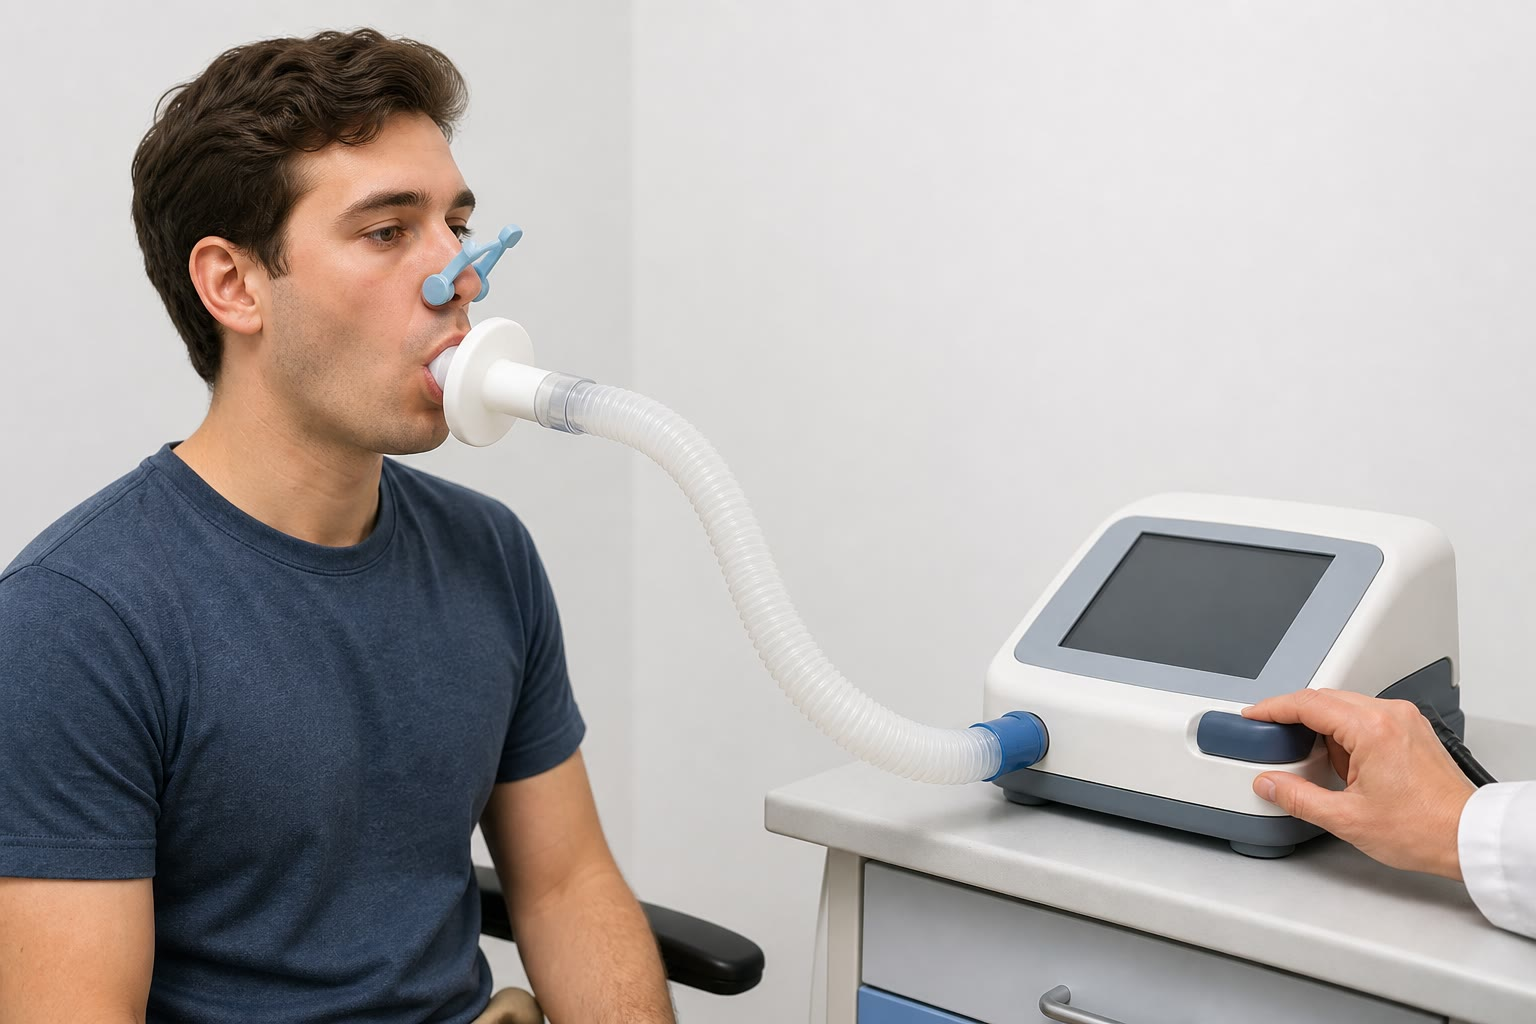
\includegraphics[width=0.58\linewidth]{images/book2/ai/g10-lungs-spirometer.jpg}

{\small Medir os volumes pulmonares: o sujeito respira por um bocal
dentro de um espirômetro, com o nariz preso por um clipe, e o
instrumento registra o volume de cada incursão.}
\end{omfigure}

\section{O coração e as duas circulações}

\begin{definition}[Débito cardíaco]\label{def:g10:heart-lungs-effort:output}
O coração é uma bomba dupla de quatro câmaras. O lado direito recebe o
sangue que volta dos órgãos e o manda para os pulmões (a
\emph{circulação pulmonar}); o lado esquerdo o recebe de volta dos
pulmões e o manda para os órgãos (a \emph{circulação sistêmica}). As
valvas entre as câmaras e nas saídas fazem o fluxo correr num sentido
só. O \emph{débito cardíaco}\index{débito cardíaco} $Q$ é o volume de
sangue que cada lado bombeia por minuto: o volume ejetado por
batimento, o \emph{volume sistólico} $V_s$, multiplicado pela
\emph{frequência cardíaca} $f$,
\[
Q = f \times V_s .
\]
Em repouso, $70$ batimentos por minuto de \qty{70}{mL}: cerca de
\qty{5}{L/min} --- todo o volume de sangue uma vez por minuto.
\end{definition}

\begin{omfigure}
\begin{tikzpicture}[>=Stealth, font=\small,
  ch/.style={draw, thick, rounded corners, minimum width=1.9cm, minimum height=1.0cm, align=center},
  org/.style={draw, thick, rounded corners, minimum width=2.6cm, minimum height=1.0cm, align=center}]
  \node[org, fill=omDef!15] (lungs) at (3.5,3.6) {pulmões};
  \node[ch, fill=omDef!25] (ra) at (0.7,1.2) {átrio\\ direito};
  \node[ch, fill=omDef!25] (rv) at (0.7,0) {ventrículo\\ direito};
  \node[ch, fill=omThm!20] (la) at (6.3,1.2) {átrio\\ esquerdo};
  \node[ch, fill=omThm!20] (lv) at (6.3,0) {ventrículo\\ esquerdo};
  \node[org, fill=omThm!12] (org) at (3.5,-2.8) {músculos e\\ outros órgãos};
  \draw[->, thick, omDef] (ra) -- (rv);
  \draw[->, thick, omDef, rounded corners=6pt] (rv.west) -- (-1.55,0) -- (-1.55,3.6) -- (lungs.west);
  \node[anchor=east, align=right, omDef] at (-1.7,2.4) {artéria\\ pulmonar};
  \draw[->, thick, omThm, rounded corners=6pt] (lungs.east) -- (8.6,3.6) -- (8.6,1.2) -- (la.east);
  \node[anchor=west, align=left, omThm] at (8.75,2.4) {veias\\ pulmonares};
  \draw[->, thick, omThm] (la) -- (lv);
  \draw[->, thick, omThm, rounded corners=6pt] (lv.east) -- (8.6,0) -- (8.6,-2.8) -- (org.east);
  \node[anchor=west, omThm] at (8.75,-1.4) {aorta};
  \draw[->, thick, omDef, rounded corners=6pt] (org.west) -- (-2.3,-2.8) -- (-2.3,1.2) -- (ra.west);
  \node[anchor=east, omDef] at (-2.45,-1.4) {veias};
  \node[font=\small, anchor=north, text width=3.2cm, align=center] at (3.5,-3.6) {oxigênio sai, $\mathrm{CO_2}$ entra};
  \node[font=\small, anchor=south, text width=3.2cm, align=center] at (3.5,4.2) {oxigênio entra, $\mathrm{CO_2}$ sai};
  \draw[thick, dashed, gray] (3.5,2.5) -- (3.5,-1.9);
\end{tikzpicture}

{\small A circulação dupla. Em azul: sangue pobre em oxigênio,
bombeado pelo coração direito para os pulmões. Em vermelho: sangue rico
em oxigênio, bombeado pelo coração esquerdo para os órgãos. Os dois
lados batem juntos e bombeiam o mesmo volume por minuto.}
\end{omfigure}

\begin{proposition}[O débito cardíaco durante o exercício]\label{prop:g10:heart-lungs-effort:output-exercise}
Durante o exercício a frequência cardíaca sobe com a potência
entregue, até um máximo de aproximadamente $220$ menos a idade em anos,
e o volume sistólico também sobe, cerca de metade numa pessoa não
treinada e mais numa treinada. O \omterm{def:g10:heart-lungs-effort:output}{débito cardíaco} de um adulto jovem vai
de \qty{5}{L/min} em repouso a \qtyrange{20}{25}{L/min} no esforço
máximo, e a \qty{35}{L/min} ou mais num campeão de provas de
resistência, cujo volume sistólico pode passar de \qty{180}{mL}.
\end{proposition}
\admitted

\begin{omfigure}
\begin{tikzpicture}
\begin{axis}[
  width=0.86\linewidth, height=5.8cm,
  axis x line=bottom, axis y line=left,
  xmin=0, xmax=320, ymin=0, ymax=210,
  xlabel={potência mecânica (W)}, ylabel={frequência cardíaca (por min), volume sistólico (mL)},
  xlabel style={font=\small, at={(axis description cs:0.5,-0.12)}, anchor=north},
  ylabel style={font=\small},
  tick label style={font=\small},
  xtick={0,50,100,150,200,250,300}, ytick={0,50,100,150,200},
  legend style={at={(0.5,-0.3)}, anchor=north, legend columns=3, font=\small, draw=none},
  clip=false,
]
\addplot[thick, omThm, mark=*, mark size=1.5pt] coordinates
  {(0,70) (50,95) (100,120) (150,145) (200,170) (250,190) (300,198)};
\addplot[thick, omDef, mark=square*, mark size=1.5pt] coordinates
  {(0,70) (50,90) (100,105) (150,112) (200,115) (250,115) (300,115)};
\addplot[thick, omMeth, dashed, mark=triangle*, mark size=1.8pt] coordinates
  {(0,4.9) (50,8.6) (100,12.6) (150,16.2) (200,19.6) (250,21.9) (300,22.8)};
\legend{frequência cardíaca, volume sistólico, débito (L/min)}
\end{axis}
\end{tikzpicture}

{\small Frequência cardíaca, volume sistólico e \omterm{def:g10:heart-lungs-effort:output}{débito cardíaco} de um
jovem de vinte anos em potência crescente. O volume sistólico se
estabiliza no esforço moderado; acima disso o débito sobe apenas pela
frequência, e a própria frequência se estabiliza perto de
$220 - 20 = 200$.}
\end{omfigure}

\begin{example}[O débito a \qty{200}{W}]\label{ex:g10:heart-lungs-effort:output200}
Pela figura: $f = 170$ por minuto, $V_s = \qty{115}{mL}$, logo
$Q = 170 \times 0.115 \approx \qty{19.6}{L/min}$: quatro vezes o débito
de repouso. O coração está movendo todo o volume de sangue do corpo
quatro vezes por minuto.
\end{example}

\section{Levar o sangue aonde ele é preciso}

\begin{proposition}[Redistribuição do fluxo sanguíneo]\label{prop:g10:heart-lungs-effort:redistribution}
Em repouso os músculos recebem cerca de um quinto do \omterm{def:g10:heart-lungs-effort:output}{débito cardíaco}; o
intestino, o fígado e os rins ficam com metade. Durante um exercício
intenso as pequenas artérias dos músculos em atividade se dilatam e as
do intestino e dos rins se estreitam: os músculos passam então a
receber mais de quatro quintos de um débito que ele próprio
quadruplicou --- uns \qty{20}{L/min} em vez de \qty{1}{L/min}, vinte
vezes mais. A parcela do cérebro é mantida constante em termos
absolutos, e a da pele sobe para levar o calor embora.
\end{proposition}
\admitted

\begin{omfigure}
\begin{tikzpicture}
\begin{axis}[
  xbar stacked, bar width=15pt,
  width=0.86\linewidth, height=3.8cm,
  axis x line=bottom, axis y line=left,
  xmin=0, xmax=25, xlabel={fluxo sanguíneo (L/min)},
  xlabel style={font=\small, at={(axis description cs:0.5,-0.3)}, anchor=north},
  symbolic y coords={repouso, exercício máximo},
  ytick=data, tick label style={font=\small},
  enlarge y limits=0.5,
  legend style={at={(0.5,-0.65)}, anchor=north, legend columns=5, font=\small, draw=none},
]
\addplot[fill=omThm!50, draw=omThm] coordinates {(1.0,repouso) (20.5,exercício máximo)};
\addplot[fill=omProp!50, draw=omProp] coordinates {(2.5,repouso) (0.9,exercício máximo)};
\addplot[fill=omDef!50, draw=omDef] coordinates {(0.75,repouso) (0.75,exercício máximo)};
\addplot[fill=gray!40, draw=gray] coordinates {(0.5,repouso) (1.2,exercício máximo)};
\addplot[fill=omMeth!50, draw=omMeth] coordinates {(0.25,repouso) (0.65,exercício máximo)};
\legend{músculos, intestino e rins, cérebro, pele, outros}
\end{axis}
\end{tikzpicture}

{\small Para onde vai o \omterm{def:g10:heart-lungs-effort:output}{débito cardíaco}, em repouso (\qty{5}{L/min}) e
no exercício máximo (\qty{24}{L/min}). A parcela dos músculos vai de um
quinto a mais de quatro quintos; o cérebro mantém os \qty{0.75}{L/min}
dele o tempo todo.}
\end{omfigure}

\begin{proposition}[Entrega e extração de oxigênio]\label{prop:g10:heart-lungs-effort:extraction}
Cada litro de sangue arterial carrega cerca de \qty{200}{mL} de
oxigênio, quase todo ligado à hemoglobina das hemácias. Em repouso os
órgãos retiram cerca de \qty{50}{mL} de cada litro; durante o exercício
os músculos em atividade retiram até \qty{150}{mL}, três vezes mais. O
oxigênio consumido por minuto é o \omterm{def:g10:heart-lungs-effort:output}{débito cardíaco} multiplicado pela
quantidade retirada por litro --- de modo que a subida de cinco vezes
do débito e a de três vezes da extração dão juntas a subida de quinze
vezes no consumo de oxigênio do \cref{ch:g10:exercise-and-energy}.
\end{proposition}
\admitted

\begin{example}[O balanço do oxigênio conferido]\label{ex:g10:heart-lungs-effort:fick}
Repouso: \qty{5}{L/min} $\times$ \qty{50}{mL/L} $= \qty{250}{mL/min}$,
o consumo de repouso. Esforço máximo de um estudante treinado:
\qty{23}{L/min} $\times$ \qty{150}{mL/L} $= \qty{3.45}{L/min}$ --- um
$\dot V\!\mathrm{O_2}$max de \qty{50}{mL/min} por quilograma para
\qty{69}{kg}, exatamente o número do capítulo anterior.
\end{example}

\section{Como a resposta é comandada}

\begin{proposition}[Controle nervoso e hormonal]\label{prop:g10:heart-lungs-effort:control}
O coração e os músculos respiratórios são comandados por centros
nervosos da base do encéfalo. Dois conjuntos de nervos chegam ao
coração: um o desacelera, ativo em repouso; outro o acelera e reforça
cada batimento. No início do exercício a ordem do encéfalo aos músculos
é copiada para esses centros --- o coração acelera em um ou dois
batimentos --- e sensores dos músculos e das articulações informam o
movimento. Depois, conforme o exercício continua, sensores das artérias
medem o gás carbônico e a acidez do sangue e ajustam a \omterm{def:g10:heart-lungs-effort:ventilation}{ventilação} e a
frequência cardíaca para mantê-los perto dos valores de repouso. As
glândulas suprarrenais acrescentam o hormônio
\emph{adrenalina}\index{adrenalina}, que reforça a aceleração e dilata
as artérias dos músculos.
\end{proposition}
\begin{proof}[Evidências]
Cortar o nervo desacelerador de um animal eleva a frequência cardíaca
de repouso dele de 70 para cerca de 100; estimulá-lo faz o coração
parar. Estimular o nervo acelerador dobra a frequência. Uma pessoa
avisada de que vai fazer um esforço mostra a frequência cardíaca
subindo antes de se mover; um sujeito que respira ar enriquecido em gás
carbônico aumenta a \omterm{def:g10:heart-lungs-effort:ventilation}{ventilação} em menos de um minuto, e um sujeito cujo
gás carbônico do sangue é mantido constante artificialmente durante o
exercício ainda assim a aumenta no início do movimento --- os dois
mecanismos, a antecipação e a correção, são ambos reais.
\end{proof}

\begin{method}[Calcular a entrega de oxigênio]\label{met:g10:heart-lungs-effort:compute}
\begin{enumerate}
  \item \omterm{def:g10:heart-lungs-effort:ventilation}{Ventilação}: volume corrente $\times$ frequência. Só cerca de
        70\% de cada incursão chega aos \omterm{def:g10:heart-lungs-effort:ventilation}{alvéolos}; o resto preenche as
        vias aéreas.
  \item \omterm{def:g10:heart-lungs-effort:output}{Débito cardíaco}: $Q = f \times V_s$, em litros por minuto se
        $V_s$ estiver em litros.
  \item Oxigênio consumido por minuto: $Q \times$ (oxigênio retirado
        por litro de sangue).
  \item Fluxo até um órgão: a parcela dele em $Q$. Compare fluxos
        absolutos, não parcelas --- uma parcela menor de um débito
        maior pode ser mais sangue.
  \item Confira: o consumo não pode ultrapassar o
        $\dot V\!\mathrm{O_2}$max, e $f$ não pode ultrapassar cerca de
        $220 - $ a idade.
\end{enumerate}
\end{method}

\begin{remark}[Onde está o limite]\label{rem:g10:heart-lungs-effort:limit}
A \omterm{def:g10:heart-lungs-effort:ventilation}{ventilação} pode passar de \qty{150}{L/min} e o sangue que sai dos
pulmões continua quase saturado no esforço máximo: os pulmões não são o
gargalo. O volume sistólico é: ele fixa quanto sangue, e portanto
quanto oxigênio, cada batimento entrega. O treinamento de resistência
aumenta o coração e o volume sistólico dele --- e é por isso que um
coração treinado em repouso bate a 45 em vez de 70 para os mesmos
\qty{5}{L/min}, e por que o $\dot V\!\mathrm{O_2}$max sobe com o
treinamento.
\end{remark}

\section{Exercícios}

\begin{exercise}[$\star$]\label{exo:g10:heart-lungs-effort:1}
Calcule a \omterm{def:g10:heart-lungs-effort:ventilation}{ventilação} de uma pessoa que respira \qty{0.6}{L} catorze
vezes por minuto; depois a da mesma pessoa respirando \qty{2.2}{L}
trinta e cinco vezes por minuto.
\end{exercise}

\begin{exercise}[$\star$]\label{exo:g10:heart-lungs-effort:2}
Defina \omterm{def:g10:heart-lungs-effort:output}{débito cardíaco} e dê a fórmula dele. Calcule-o para uma
frequência cardíaca de 65 por minuto e um volume sistólico de
\qty{75}{mL}.
\end{exercise}

\begin{exercise}[$\star$]\label{exo:g10:heart-lungs-effort:3}
Trace o caminho de uma hemácia do átrio direito de volta ao átrio
direito, nomeando as câmaras e as duas circulações.
\end{exercise}

\begin{exercise}[$\star$]\label{exo:g10:heart-lungs-effort:4}
A partir da figura do espirograma, dê o volume corrente, a capacidade
vital e o volume residual.
\end{exercise}

\begin{exercise}[$\star$]\label{exo:g10:heart-lungs-effort:5}
Qual é a frequência cardíaca máxima de alguém de 16 anos? E de 60 anos?
\end{exercise}

\begin{exercise}[$\star\star$]\label{exo:g10:heart-lungs-effort:6}
A partir da figura da frequência cardíaca, calcule o \omterm{def:g10:heart-lungs-effort:output}{débito cardíaco} a
\qty{100}{W} e a \qty{300}{W}, e o fator entre os dois.
\end{exercise}

\begin{exercise}[$\star\star$]\label{exo:g10:heart-lungs-effort:7}
Em repouso o intestino e os rins recebem 50\% de \qty{5}{L/min}; no
exercício máximo, 4\% de \qty{24}{L/min}. Calcule os dois fluxos. O que
muda mais, a parcela ou o fluxo absoluto?
\end{exercise}

\begin{exercise}[$\star\star$]\label{exo:g10:heart-lungs-effort:8}
Uma pessoa tem um \omterm{def:g10:heart-lungs-effort:output}{débito cardíaco} de \qty{18}{L/min} e os músculos dela
retiram \qty{140}{mL} de oxigênio por litro. Calcule o consumo de
oxigênio dela. Ela está perto do teto de uma estudante treinada?
\end{exercise}

\begin{exercise}[$\star\star$]\label{exo:g10:heart-lungs-effort:9}
Por que o fluxo sanguíneo do cérebro permanece em \qty{0.75}{L/min}
enquanto o do intestino é cortado em dois terços durante o exercício?
Pense no que cada órgão consegue tolerar.
\end{exercise}

\begin{exercise}[$\star\star$]\label{exo:g10:heart-lungs-effort:10}
Uma ciclista treinada tem frequência cardíaca de repouso de 42 e débito
de repouso de \qty{5}{L/min}. Calcule o volume sistólico dela e compare
com o de uma pessoa não treinada.
\end{exercise}

\begin{exercise}[$\star\star$]\label{exo:g10:heart-lungs-effort:11}
Explique por que a frequência cardíaca começa a subir antes do primeiro
passo de uma corrida, e o que aconteceria a um corredor cujo controle
funcionasse apenas detectando o gás carbônico do sangue.
\end{exercise}

\begin{exercise}[$\star\star\star$]\label{exo:g10:heart-lungs-effort:12}
Dois sujeitos alcançam a mesma frequência cardíaca máxima de 195. Um
tem volume sistólico máximo de \qty{110}{mL}, o outro de
\qty{160}{mL}. Com a mesma extração de oxigênio de \qty{150}{mL/L},
calcule os \omterm{def:g10:exercise-and-energy:vo2max}{consumos máximos de oxigênio} deles, e diga o que a
\cref{rem:g10:heart-lungs-effort:limit} prevê sobre o histórico de
treinamento de cada um.
\end{exercise}

\begin{exercise}[$\star\star\star$]\label{exo:g10:heart-lungs-effort:13}
O ar é 21\% oxigênio. Uma pessoa ventila \qty{100}{L/min} no esforço
máximo e consome \qty{3.5}{L/min} de oxigênio. Que fração do oxigênio
que ela inspira ela realmente usa? O que o resto faz?
\end{exercise}

\begin{exercise}[$\star\star\star$]\label{exo:g10:heart-lungs-effort:14}
Um medicamento bloqueia os nervos aceleradores e o efeito da
\omterm{prop:g10:heart-lungs-effort:control}{adrenalina} sobre o coração, limitando a frequência cardíaca a 110.
Preveja o efeito disso sobre o \omterm{def:g10:heart-lungs-effort:output}{débito cardíaco} no esforço máximo, sobre
o $\dot V\!\mathrm{O_2}$max e sobre o que o paciente consegue fazer.
\end{exercise}

\begin{exercise}[$\star\star\star$]\label{exo:g10:heart-lungs-effort:15}
Uma pessoa em grande altitude tem sangue arterial que carrega
\qty{150}{mL} de oxigênio por litro em vez de \num{200}. Com o mesmo
\omterm{def:g10:heart-lungs-effort:output}{débito cardíaco} máximo e a mesma extração de 75\% do oxigênio entregue,
calcule a perda de $\dot V\!\mathrm{O_2}$max em por cento. Proponha uma
adaptação que o corpo faz nas semanas seguintes.
\end{exercise}

\section{Problema: o teste de esforço}

\begin{problem}[{Problema de fim de semana --- o teste de esforço de um
cardiologista: frequência cardíaca, volume sistólico, ventilação e
extração de oxigênio medidos em potência crescente, e a multiplicação
que eles alcançam juntos}]
\label{pb:g10:heart-lungs-effort:1}
Tom, 17 anos, massa de \qty{68}{kg}, pedala numa bicicleta de
laboratório enquanto a frequência cardíaca, a \omterm{def:g10:heart-lungs-effort:ventilation}{ventilação} e o ar
expirado dele são registrados. Resultados:

\begin{center}
\begin{tabular}{lccccc}
potência (W) & 0 & 75 & 150 & 225 & 300 \\ \hline
frequência cardíaca (por min) & 62 & 105 & 140 & 175 & 198 \\
volume sistólico (mL) & 72 & 100 & 116 & 120 & 120 \\
volume corrente (L) & 0.5 & 1.2 & 1.8 & 2.3 & 2.6 \\
incursões por min & 13 & 18 & 24 & 32 & 44 \\
$\mathrm{O_2}$ retirado por litro de sangue (mL) & 52 & 90 & 120 & 145 & 155 \\
\end{tabular}
\end{center}

\medskip
\noindent\textbf{Parte I --- O coração.}
\begin{enumerate}
  \item Calcule o \omterm{def:g10:heart-lungs-effort:output}{débito cardíaco} de Tom em cada potência.
  \item Por que fator o débito subiu a \qty{300}{W}? Que parte desse
        fator vem da frequência e que parte vem do volume sistólico?
  \item Acima de que potência o volume sistólico para de subir? O que,
        sozinho, aumenta o débito a partir daí?
  \item Compare a frequência cardíaca máxima de Tom com a regra
        prática.
  \item O débito de repouso dele é de cerca de \qty{4.5}{L/min}. Se o
        volume de sangue dele é de \qty{5}{L}, quanto tempo leva uma
        volta completa em repouso, e a \qty{300}{W}?
\end{enumerate}

\medskip
\noindent\textbf{Parte II --- Os pulmões.}
\begin{enumerate}[resume]
  \item Calcule a \omterm{def:g10:heart-lungs-effort:ventilation}{ventilação} em cada potência.
  \item Por que fator ela subiu a \qty{300}{W}? Qual dos dois fatores,
        o volume ou a frequência, contribui mais?
  \item A capacidade vital de Tom é de \qty{5.0}{L}. Que fração dela
        cada incursão usa a \qty{300}{W}?
  \item A \omterm{def:g10:heart-lungs-effort:ventilation}{ventilação} subiu por um fator maior que o \omterm{def:g10:heart-lungs-effort:output}{débito cardíaco}.
        Isso quer dizer que os pulmões limitam o desempenho? Use a
        \cref{rem:g10:heart-lungs-effort:limit}.
  \item Só 70\% de cada incursão chega aos \omterm{def:g10:heart-lungs-effort:ventilation}{alvéolos}. Calcule a
        \omterm{def:g10:heart-lungs-effort:ventilation}{ventilação} alveolar em repouso e a \qty{300}{W}.
\end{enumerate}

\medskip
\noindent\textbf{Parte III --- O oxigênio.}
\begin{enumerate}[resume]
  \item Calcule o consumo de oxigênio de Tom em cada potência, a
        partir do \omterm{def:g10:heart-lungs-effort:output}{débito cardíaco} e do oxigênio retirado por litro.
  \item Expresse o valor a \qty{300}{W} em mililitros por minuto por
        quilograma. Isso é um $\dot V\!\mathrm{O_2}$max, e de que tipo
        de pessoa?
  \item Por que fator o consumo subiu do repouso até \qty{300}{W}?
        Separe-o no fator vindo do coração e no fator vindo da
        extração.
  \item Usando \qty{20}{kJ} por litro de oxigênio, calcule a potência
        metabólica a \qty{300}{W} e o rendimento dos músculos
        (potência mecânica dividida pela potência metabólica acima do
        repouso).
  \item Trace, ou descreva, o consumo de oxigênio em função da
        potência mecânica. É linear? Onde está o teto?
\end{enumerate}

\medskip
\noindent\textbf{Parte IV --- O controle e o veredito.}
\begin{enumerate}[resume]
  \item A frequência cardíaca de Tom chegou a 75 enquanto ele estava
        sentado esperando o teste começar. Explique.
  \item A \qty{300}{W} o sangue arterial dele ainda está 95\% saturado
        de oxigênio. O que isso diz a você sobre a troca nos \omterm{def:g10:heart-lungs-effort:ventilation}{alvéolos} e
        sobre onde está o limite do $\dot V\!\mathrm{O_2}$max dele?
  \item O cardiologista anota que os músculos agora recebem cerca de
        \qty{20}{L/min} de sangue. Que fração do débito é isso, e para
        onde foi o resto da distribuição de repouso?
  \item Depois de seis meses de treinamento, o volume sistólico máximo
        de Tom é de \qty{140}{mL} com a mesma frequência máxima e a
        mesma extração. Calcule o novo $\dot V\!\mathrm{O_2}$max dele.
  \item Enuncie o resultado: os três números (coração, extração,
        \omterm{def:g10:heart-lungs-effort:ventilation}{ventilação}) pelos quais o corpo de Tom multiplicou o
        fornecimento de oxigênio de repouso, e o único deles que o
        treinamento mudou.
\end{enumerate}
\end{problem}
